%
% chapter.tex -- Nicht differenzierbare Lösungen
%
% (c) 2023 Prof Dr Andreas Müller
%
\chapter{Nicht differenzierbare Lösungen
\label{buch:chapter:nichtdiff}}
\kopflinks{Nicht differenzierbare Lösungen}
Die Herleitung der Euler-Lagrange-Differentialgleichung im
Abschnitt~\ref{buch:variation:euler-lagrange} hat vorausgesetzt,
dass die Lösungsfunktion mindestens zweimal stetig differenzierbar ist.
Dies war nötig, um die partielle Integration durchführen zu können,
schränkt aber auch die Menge der Kandidatenfunktionen für die Lösungen
stark ein.
Im Abschnitt~\ref{buch:nichtdiff:section:duboisreymond} wird 
das Lemma von du~Bois-Reymond vorgestellt, welches eine alternative
Vorgehensweise zeigt, mit der die Ableitung vermieden werden kann.

Es liegt jedoch in der Natur von Variationsproblemen, dass sie 
als Lösungen nicht differenzierbare Lösungen haben können.
Das Lemma von du~Bois-Reymond beseitigt diese Schwierigkeit
nicht, es werden nur die Anforderungen an die Funktionen auf 
nur eine Ableitung abgeschwächt.
Die Weierstrass-Ermdannsche Eckenbedingung, die in
Abschnitt~\ref{buch:nichtdiff:section:ecken} vorgestellt
wird, ermöglicht, Lösungsfunktionen zu finden, welche mit Ausnahme
einiger diskreter Stellen Lösungen der Euler-Lagrange-Differentialgleichung
sind.
An dien Ausnahmestellen sind die Lösungen immer noch stetig, die
Ableitung kann aber springen, jedoch nicht beliebig.

Die im Abschnitt~\ref{buch:nichtdiff:section:splines} vorgestellte,
für die numerische Mathematik besonders wichtige
Spline-Interpolation verwendet Lösungsfunktionen eines
Variationsproblems zur Approximation einer Funktion, welche aber an
einigen Stellen nicht stetig differenzierbar sind.


%
% 1-duboisreymond.tex
%
% (c) 2024 Prof Dr Andreas Müller
%
\section{Das Lemma von du~Bois-Reymond
\label{buch:nichtdiff:section:duboisreymond}}
\kopfrechts{Das Lemma von du~Bois-Reymond}
Wir gehen wieder von einem Variationsproblem der Form
\begin{equation}
\delta
\int_{x_0}^{x_1}
F(x,y(x),y'(x))\,dx
=
0
\label{buch:nichtdiff:duboisreymond:eqn:problem}
\end{equation}
mit festen Randwerten $y(x_0)=y_0$ und $y(x_1)=y_1$ aus.
Die Herleitung der Euler-Lagrange-Differentialgleichung für dieses
Problem hat angenommen, dass die Lösungsfunktion $y(x)$ zweimal
stetig differenzierbar ist.
Paul du~Bois-Reymond%
\footnote{Paul du~Bois-Reymond, 1831--1889, deutscher
Mathematiker, studierte erst in Zürich Medizin, dann in Mathematik
in Königsberg und an der Universität Berlin.
Er promovierte bei Ernst Kummer und arbeitete anschliessend als
Gymnasiallehrer.
Er habilitierte sich 1865 in Heidelberg und 1869 als Professor nach
Freiburg im  Breisgau berufen.
Ab 1874 wirkte er in Tübingen und ab 1884 an der
Technischen Hochschule Berlin.}
hat darauf hingewiesen, dass dadurch die Menge der akzeptablen
Lösungsfunktionen unnötig eingeschränkt wird.
Die folgende Rechnung und das weiter unten formulierte 
Lemma~\ref{buch:nichtdiff:duboisreymond:lemma:duboisreymond}
zeigen, dass die Euler-Lagrange-Gleichung auch gilt, wenn $y(x)$
als nur einmal stetig differenzierbar angenommen wird.

Die erste Variation ist die Ableitung
\[
\frac{d}I(y+\varepsilon\eta)\bigg|_{\varepsilon=0}
=
\frac{d}{d\varepsilon}
\int_{x_0}^{x_1}
F(x,y(x)+\varepsilon\eta(x), y'(x)+\varepsilon\eta'(x))\,dx
\bigg|_{\varepsilon}
\]
für beliebige Variationen $\eta(x)$ der Funktion $y(x)$.
Wie früher nehmen wir an, dass $F$ nach $y$ und $y'$ differenzierbar
ist, und verwenden dies, um die Ableitung zu berechnen:
\begin{equation}
\frac{d}{d\varepsilon}I(y+\varepsilon\eta)
=
\int_{x_0}^{x_1}
\frac{\partial F}{\partial y}(x,y(x),y'(x))\cdot \eta(x)
+
\frac{\partial F}{\partial y'}(x,y(x),y'(x))\cdot \eta'(x)
\,dx.
\label{nichtdiff:duboisreymon:eqn:ableitung}
\end{equation}
Bei der Herleitung der Euler-Lagrange-Gleichung in
Abschnitt~\ref{buch:variation:section:eulerlagrange}
haben wir uns nicht gescheut, den zweiten Term im Integral
partiell zu integrieren, und aus dem Faktor $\eta'(x)$ einen
beiden Termen gemeinsamen Faktor $\eta(x)$ zu machen.
Falls jedoch $y(x)$ nicht differenzierbar ist, oder wenn $F$ nur
einmal stetig differenzierbar ist, ist dies nicht zulässig.

Es gibt aber keine solchen Einschränkungen für die Funktionen $\eta(x)$.
Wir können uns bei der Wahl von $\eta(x)$ auf beliebig oft differenzierbare
Funktionen einschränken.
Wir versuchen daher den ersten Term
in~\eqref{nichtdiff:duboisreymon:eqn:ableitung}
partiell zu integrieren.
Die dazu benötigte Stammfunktion des ersten Terms schreiben wir
\[
\int_{x_0}^x \frac{\partial F}{\partial y}(\xi, y(\xi), y'(\xi))\,d\xi.
\]
Das erste Integral in~\eqref{nichtdiff:duboisreymon:eqn:ableitung}
wird damit zu
\begin{align*}
\int_{x_0}^{x_1}
\frac{\partial F}{\partial y}(x,y(x),y'(x)\eta(x)\,dx
&=
\biggl[
\int_{x_0}^{x}
\frac{\partial F}{\partial y}(\xi,y(\xi),y'(\xi))
\,d\xi
\cdot 
\eta(x)
\biggr]_{x_0}^{x_1}
\\
&\qquad
-
\int_{x_0}^{x_1}
\int_{x_0}^{x}
\frac{\partial F}{\partial y}(\xi,y(\xi),y'(\xi))
\,d\xi
\cdot\eta'(x)
\,dx.
\end{align*}
Da in den Randpunkten $\eta(x_0)=\eta(x_1)=0$ gilt, 
fällt der erste Term weg.
Einsetzen in~\eqref{nichtdiff:duboisreymon:eqn:ableitung}
liefert jetzt die Bedingung
\begin{equation}
\int_{x_0}^{x_1}
\biggl(
-\int_{x_0}^x\frac{\partial F}{\partial y}(\xi, y(\xi),y'(\xi))
\,d\xi
+
\frac{\partial F}{\partial y'}(x,y(x),y'(x))
\biggr)
\cdot
\eta'(x)\,dx
=
0
\label{buch:nichtdiff:duboisreymond:eqn:integralgleichung}
\end{equation}
für alle einmal stetig differenzierbaren Funktionen $\eta(x)$, die
an den Endpunkten des Intervalls verschwinden.
Daraus können wir aber nicht schliessen, dass die Klammer im
Integral verschwindet, denn dies folgt nach dem Fundamentallemma
nur, wenn man mit beliebige Funktionen $\eta(x)$ multipliziert.
Die Funktionen $\eta'(x)$ haben die einschränkende Eigenschaft,
dass ihr Integral zwischen $x_0$ und $x_1$
\[
\int_{x_0}^{x_1}
\eta'(x)\,dx
=
\biggl[
\eta(x)
\biggr]_{x_0}^{x_1}
=
\eta(x_1) - \eta(x_0)
=
0-0
=
0
\]
ist.
Für beliebige Funktionen $\eta(x)$ kann das Integral zwischen $x_0$
und $x_1$ bliebige Werte annehmen, selbst wenn $\eta(x_0)=\eta(x_1)=0$
sind.
Es gilt aber die folgende Verallgemeinerung des Fundamentallemmas.

\begin{lemma}[du Bois-Reymond
\footnote{Paul du~Bois-Reymond, 1831--1889, deutscher
Mathematiker, studierte erst in Zürich Medizin, dann in Mathematik
in Königsberg und an der Universität Berlin.
Er promovierte bei Ernst Kummer und arbeitete anschliessend als
Gymnasiallehrer.
Er habilitierte sich 1865 in Heidelber und 1869 als Professor nach
Freiburg im  Breisgau berufen.
Ab 1874 wirkte er in Tübingen und ab 1884 an der
Technischen Hochschule Berlin.}]
\label{buch:nichtdiff:duboisreymond:lemma:duboisreymond}
Sei $f(x)$ eine stetige Funktion auf dem Intervall $[x_0,x_1]$, für die
\[
\int_{x_0}^{x_1}
f(x)\,\eta'(x)\,dx
=
0
\]
gilt für alle einmal stetig differenzierbaren Funktionen auf $[x_0,x_1]$,
die in den Intervallenden verschwinden.
Dann ist die Funktion $f(x)$ konstant.
\end{lemma}

%
% dbr.tex -- Beweis des Lemmas von du Bois-Reymond
%
% (c) 2024 Prof Dr Andreas Müller, OST Ostschweizer Fachhochschule
%
\documentclass[tikz]{standalone}
\usepackage{amsmath}
\usepackage{times}
\usepackage{txfonts}
\usepackage{pgfplots}
\usepackage{csvsimple}
\definecolor{darkgreen}{rgb}{0,0.6,0}
\definecolor{darkred}{rgb}{0.8,0,0}
\usetikzlibrary{arrows,intersections,math,calc}
\begin{document}
\def\skala{1}
\begin{tikzpicture}[>=latex,thick,scale=\skala,
declare function={ f(\x) = 2*cos(10*\x-20)+0.5*sin(50*\x)+1; },
]

\def\a{2}
\def\b{8}
\def\e{0.8}
\def\h{3}
\def\d{0.45}

\fill[color=orange!20] ({\a-\e},{f(\a)-\d}) rectangle ({\a+\e},{f(\a)+\d});
\fill[color=orange!20] ({\b-\e},{f(\b)-\d}) rectangle ({\b+\e},{f(\b)+\d});
\fill[color=blue!20]
	plot[domain=-180:180] ({\a-\e*\x/180},{\h*(1+cos(\x))/2}) -- cycle;
\fill[color=darkred!20]
	plot[domain=-180:180] ({\b-\e*\x/180},{-\h*(1+cos(\x))/2}) -- cycle;

\draw[color=orange,line width=1.4pt] ({\a-\e},{f(\a)}) -- ({\a+\e},{f(\a)});
\draw[color=orange,line width=1.4pt] ({\b-\e},{f(\b)}) -- ({\b+\e},{f(\b)});
\draw[color=orange,line width=0.4pt]
	({\a-\e},0) -- ({\a-\e},{f(\a)}) -- ({\a+\e},{f(\a)}) -- ({\a+\e},0);
\draw[color=orange,line width=0.4pt]
	({\b-\e},0) -- ({\b-\e},{f(\b)}) -- ({\b+\e},{f(\b)}) -- ({\b+\e},0);

\draw[color=darkgreen,line width=1.4pt]
	plot[domain=0:11,samples=100] ({\x},{f(\x)});
\draw[color=darkgreen,line width=0.3pt] (\a,0) -- (\a,{f(\a)});
\draw[color=darkgreen,line width=0.3pt] (\b,0) -- (\b,{f(\b)});
\fill[color=darkgreen] (\a,{f(\a)}) circle[radius=0.08];
\fill[color=darkgreen] (\b,{f(\b)}) circle[radius=0.08];
\node[color=darkgreen] at (\a,{f(\a)}) [above] {$f(a)$};
\node[color=darkgreen] at (\b,{f(\b)}) [above] {$f(b)$};

\node[color=orange] at ({\a+\e},{f(\a)+\d}) [right] {$f(a)+\delta\mathstrut$};
\node[color=orange] at ({\a+\e},{f(\a)-\d}) [right] {$f(a)-\delta\mathstrut$};
\node[color=orange] at ({\b+\e},{f(\b)+\d}) [right] {$f(b)+\delta\mathstrut$};
\node[color=orange] at ({\b+\e},{f(\b)-\d}) [right] {$f(b)-\delta\mathstrut$};

\coordinate (A) at (6,3.9);

\node[color=orange] at (A) {$\tilde{f}(x)$};
\draw[color=orange,line width=0.3pt,shorten >= 0.3cm]
	({\a+0.8*\e},{f(\a)}) -- (A);
\draw[color=orange,line width=0.3pt,shorten >= 0.3cm]
	({\b-0.8*\e},{f(\b)}) -- (A);

\node[color=darkgreen] at (5,{f(5)}) [below] {$f(x)$};

\draw[color=blue,line width=1.1pt]
	plot[domain=-180:180] ({\a-\e*\x/180},{\h*(1+cos(\x))/2});

\draw[color=darkred,line width=1.1pt]
	plot[domain=-180:180] ({\b-\e*\x/180},{-\h*(1+cos(\x))/2});

\draw[->] (-0.1,0) -- (11.5,0) coordinate[label={$x$}];
\draw[->] (0,-3.2) -- (0,4.3) coordinate[label={left:$y$}];

\draw (\a,-0.05) -- (\a,0.05);
\node at (\a,0) [below] {$a\mathstrut$};
\draw (\b,-0.05) -- (\b,0.05);
\node at (\b,0) [below] {$b\mathstrut$};

\draw ({\a-\e},-0.05) -- ({\a-\e},0.05);
\node at ({\a-\e},0) [below left] {$a-\varepsilon\mathstrut$};
\draw ({\a+\e},-0.05) -- ({\a+\e},0.05);
\node at ({\a+\e},0) [below right] {$a+\varepsilon\mathstrut$};

\node[color=blue] at (\a,{0.3*\h}) {$g_a(x)$};
\node[color=darkred] at (\b,{-0.3*\h}) {$-g_b(x)$};

\draw ({\b-\e},-0.05) -- ({\b-\e},0.05);
\node at ({\b-\e},0) [below left] {$b-\varepsilon\mathstrut$};
\draw ({\b+\e},-0.05) -- ({\b+\e},0.05);
\node at ({\b+\e},0) [below right] {$b+\varepsilon\mathstrut$};

\end{tikzpicture}
\end{document}



\begin{proof}
Wir müssen zeigen, dass die Funktionswerte von $f$ in den Punkten $a$ und $b$
im inneren des Intervalls $[x_0,x_1]$ gleich gross sind.
Sei $\varepsilon>0$ so klein, dass die die Intervalle
$(a-\varepsilon,a+\varepsilon)$ und $(b-\varepsilon,b+\varepsilon)$ ebenfalls
vollständig in $[a,b]$ enthalten sind.
Nach Satz~\ref{buch:variation:satz:gabeins} gibt es zwei nichtnegative
Funktionen $g_a$ und $g_b$ mit
\[
\operatorname{supp} g_a = (a-\varepsilon,a+\varepsilon)
\qquad\text{und}\qquad
\operatorname{supp} g_b = (b-\varepsilon,b+\varepsilon),
\]
deren Integral ausserdem den Wert $1$ haben.
Wir wählen für $\eta$ die Stammfunktion
\[
\eta(x)
=
\int_{x_0}^x g_a(\xi)-g_b(\xi)\,d\xi
\]
von $x\mapsto g_a(x) -g_b(x)$.
Am linken Rand $x_0$ verschwindet sie, am rechten Rand gilt
\[
\eta(x_1)
=
\int_{x_0}^{x_1}
g_a(\xi)-g_b(\xi)
\,d\xi
=
\int_{x_0}^{x_1}
g_a(\xi)
\,d\xi
-
\int_{x_0}^{x_1}
g_b(\xi)
\,d\xi
=
1-1
=
0.
\]
Die Ableitung $\eta'(x)=g_a(x)-g_b(x)$ ist somit eine Funktion,
auf die die Voraussetzungen des Satzes zutreffend sind.
Daher gilt $\langle f,\eta'\rangle=0$.

Da die Funktion $f(x)$ stetig ist, können wir zu jedem beliebigen 
$\delta>0$ das $\varepsilon>0$ so klein wählen, dass 
$|f(x)-f(a)|<\delta$ für $|x-a|<\varepsilon$ und
$|f(x)-f(b)|<\delta$ für $|x-b|<\varepsilon$.
Wir approximieren die $f$ durch die Funktion
\[
\tilde{f}(x)
=
\begin{cases}
f(a)&\qquad x\in[a-\varepsilon,a+\varepsilon]\\
f(b)&\qquad x\in[b-\varepsilon,b+\varepsilon]\\
0&\qquad\text{sonst}.
\end{cases}
\]
Die Funktion $\tilde{f}$ ist immer noch integrierbar und es gilt
\[
|f(x)-\tilde{f}(x)| < \delta.
\]
Für das Integral $\langle f-\tilde{f}, \eta'\rangle$ folgt jetzt
\begin{align*}
|\langle f-\tilde{f},\eta'\rangle|
&=
\biggl|
\int_{x_0}^{x_1}
(f(x)-\tilde{f}(x))\eta'(x)
\,dx
\biggr|
\\
&\le
\int_{x_0}^{x_1}
|f(x)-\tilde{f}(x)| \cdot |\eta'(x)|
\,dx
\\
&\le 
\delta
\,
\biggl(
\int_{x_0}^{x_1} g_a(x)\,dx
+
\int_{x_0}^{x_1} g_b(x)\,dx
\biggr)
=
2\delta.
\end{align*}
Die beiden Integrale $\langle f,\eta'\rangle$ und 
$\langle \tilde{f},\eta'\rangle$ unterscheiden sich höchstens um
\begin{equation}
|\langle f,\eta'\rangle - \langle \tilde{f},\eta'\rangle|
=
|\langle f-\tilde{f},\eta' \rangle|
\le
2\delta,
\label{buch:nichtdiff:duboisreymond:eqn:ftildef}
\end{equation}
sie sind also beliebig nahe.

Die Funktion $\tilde{f}$ ist auf den beiden Teilintervallen
$(a-\varepsilon,a+\varepsilon)$ und $(b-\varepsilon,b+\varepsilon)$
konstant, das Integral kann daher sofort berechnet werden:
\begin{align*}
\langle \tilde{f},g_a\rangle
&=
\int_{a-\varepsilon}^{a+\varepsilon}
f(a) g_a(x)
\,dx
=
f(a)
&&\text{und}&
\langle \tilde{f},g_b\rangle
&=
\int_{b-\varepsilon}^{b+\varepsilon}
f(b) g_b(x)
\,dx
=
f(b),
\end{align*}
und damit
\[
\langle \tilde{f},\eta'\rangle
=
\langle \tilde{f},g_a-g_b\rangle
=
f(a)-f(b).
\]
Nach Voraussetzung ist $\langle f,\eta'\rangle=0$ und damit ist
wegen \eqref{buch:nichtdiff:duboisreymond:eqn:ftildef}
\[
|f(a)-f(b)|
=
|\langle\tilde{f},\eta'\rangle|
=
|
\underbrace{\langle f,\eta'\rangle}_{\displaystyle =0}
-
\langle \tilde{f},\eta'\rangle
|
=
|\langle f-\tilde{f},\eta'\rangle|
\le
2\delta
\]
für jedes beliebige $\delta > 0$.
Dies ist nur möglich, wenn $f(a)-f(b)=0$ ist oder $f(a)=f(b)$.
Somit hat $f$ überall im Intervall den gleichen Wert.
\end{proof}

Mit dem Lemma~\ref{buch:nichtdiff:duboisreymond:lemma:duboisreymond}
von du~Bois-Reymond kann man jetzt schliessen, dass der Integrand in
\eqref{buch:nichtdiff:duboisreymond:eqn:integralgleichung}
konstant sein muss.
Es gilt also
\begin{equation}
\int_{x_0}^x\frac{\partial F}{\partial y}(\xi, y(\xi),y'(\xi))
\,d\xi
=
\frac{\partial F}{\partial y'}(x,y(x),y'(x))
+
C
\label{buch:nichtdiff:duboisreymond:gleichung}
\end{equation}
Da die Funktionen $y(\xi)$ und $y'(\xi)$ stetig sind und auch
die Ableitung $\partial F/\partial y$ als stetig in allen Argumenten
vorausgesetzt ist, ist der Integrand auf der linken Seite eine
stetige Funktion von $\xi$.
Nach dem Hauptsatz der Infinitesimalrechnung ist das Integral
stetig differenzierbar und die Ableitung ist der Integrand.
Daher muss auch die rechte Seite stetig differenzierbar sein,
es ist also zulässig den Ableitungsoperator $d/dx$ darauf anzuwenden,
was die Gleichung
\begin{equation}
\frac{\partial F}{\partial y}(x,y(x),y'(x))
=
\frac{d}{dx}
\frac{\partial F}{\partial y'}(x,y(x),y'(x))
\label{buch:nichtdiff:duboisreymond:eqn:eulerlagrange}
\end{equation}
ergibt.
Die Gleichung
\eqref{buch:nichtdiff:duboisreymond:eqn:eulerlagrange}
ist aber wieder die Euler-Lgrange-Gleichung.
Die Voraussetzung, dass $y(x)$ zweimal stetig differenzierbar sein
muss, war also gar nicht notwendig für die Gültigkeit der
Euler-Lagrange-Gleichung.
Sie folgt auch, wenn man nur voraussetzt, dass $y(x)$ einmal stetig
differenzierbar ist.

Aus der Euler-Lagrange-Differentialgleichung folgt noch nicht, dass
die zweite Ableitung $y''(x)$ der Lösung stetig ist.
David Hilbert hat aber den folgenden Satz gezeigt.

\begin{satz}
Ist $\frac{\partial F}{\partial y'}$ differenzierbar und ist $y(x)$ eine
Lösung des Variationsproblems~\eqref{buch:nichtdiff:duboisreymond:eqn:problem},
dann ist $y''(x)$ überall dort definiert, wo
\begin{equation}
\frac{\partial^2 F}{\partial y^{\prime 2}}(x,y(x),y'(x)) \ne 0
\label{buch:nichtdiff:duboysreymond:eqn:positiv}
\end{equation}
gilt.
\end{satz}

\begin{proof}
Nach Voraussetzung ist die Ableitung von $F$ nach $y'$ differenzierbar.
Setzt man die Funktion $y(x)$ ein, ist nach 
\eqref{buch:nichtdiff:duboisreymond:gleichung}
die Funktion
\begin{equation}
x\mapsto
\frac{\partial F}{\partial y'}(x,y(x),y'(x))
\label{buch:nichtdiff:eqn:hilbertf}
\end{equation}
stetig differenzierbar.
Zur Berechnung der Ableitung von \eqref{buch:nichtdiff:eqn:hilbertf}
betrachten wir die Differenz
\begin{align*}
\Delta F
&=
\frac{\partial F}{\partial y'}(x+h,y(x+h),y'(x+h))
-
\frac{\partial F}{\partial y'}(x,y(x),y'(x))
\end{align*}
untersucht.
Die Ableitung von \eqref{buch:nichtdiff:eqn:hilbertf} ist
nach \eqref{buch:nichtdiff:duboisreymond:gleichung}
\begin{align*}
\frac{d}{dx}
\frac{\partial F}{\partial y'}(x,y(x),y'(x))
&=
\lim_{h\to 0}
\frac{\Delta F}{h}
=
\frac{\partial F}{\partial y}(x,y(x),y'(x)).
\end{align*}
Wir berechnen den Grenzwert auf eine andere Art.
Da $\partial F/\partial y'$ differenzierbar ist, kann man die Differenz
$\Delta F$ als
\begin{align*}
\Delta F
=
\frac{\partial^2 F}{\partial y'\partial x}(x,y(x),y'(x)) h
&+
\frac{\partial^2 F}{\partial y'\partial y}(x,y(x),y'(x)) \cdot (y(x+h)-y(x))
\\
&+
\frac{\partial^2 F}{\partial y^{\prime 2}}(x,y(x),y'(x)) \cdot (y'(x+h)+y'(x))
+
o(h)
\end{align*}
schreiben.
Teilen duch $h$ ergibt
\begin{align}
\frac{\Delta F}{h}
=
\frac{\partial^2 F}{\partial y'\partial x}(x,y(x),y'(x))
&+
\frac{\partial^2 F}{\partial y'\partial y}(x,y(x),y'(x))
\cdot
\frac{y(x+h)-y(x)}{h}
\label{buch:nichtdiff:eqn:hilbertlim1}
\\
&+
\frac{\partial^2 F}{\partial y^{\prime 2}}(x,y(x),y'(x))
\cdot
\frac{y'(x+h)-y'(x)}{h}
+
\frac{o(h)}{h}.
\label{buch:nichtdiff:eqn:hilbertlim2}
\end{align}
Die linke Seite konvergiert gegen die Ableitung von
\eqref{buch:nichtdiff:eqn:hilbertf}, somit muss auch die rechte Seite
konvergieren.

Die Voraussetzung \eqref{buch:nichtdiff:duboysreymond:eqn:positiv}
garantiert, dass nach dem Faktor \eqref{buch:nichtdiff:eqn:hilbertlim2}
aufgelöst werden kann.
\begin{align*}
\frac{y'(x+h)-y'(x)}{h}
&=
\frac{1}{\displaystyle
\frac{\partial^2 F}{\partial y^{\prime 2}}(x,y(x),y'(x))
}
\biggl(
\frac{\partial F}{\partial y}(x,y(x),y'(x))
-
\frac{\partial^2 F}{\partial y'\partial x}(x,y(x),y'(x))
\\
&\qquad\qquad
-
\frac{\partial F}{\partial y'}(x,y(x),y'(x))
\cdot
\frac{y(x+h)-y(x)}{h}
-
\frac{o(h)}{h}
\biggr).
\intertext{Der Differenzenquotient für $y(x)$ konvergiert gegen
$y'(x)$ und $o(h)/h$ konvergiert gegen $0$.
Somit konvergiert auch die linke Seite, sie ist die zweite Ableitung
}
y''(x)
&=
\frac{1}{\displaystyle
\frac{\partial^2 F}{\partial y^{\prime 2}}(x,y(x),y'(x))
}
\biggl(
\frac{\partial F}{\partial y}(x,y(x),y'(x))
-
\frac{\partial^2 F}{\partial y'\partial x}(x,y(x),y'(x))
\\
&\qquad\qquad
-
\frac{\partial F}{\partial y'}(x,y(x),y'(x))\cdot y'(x)
\biggr)
\end{align*}
von $y(x)$.
Damit ist der Satz bewiesen.
\end{proof}

In der Theorie der zweiten Variation von Kapitel~\ref{buch:chapter:variation2}
wird die notwendige Bedingung
\[
\frac{\partial^2 F}{\partial y^{\prime 2}}(x,y(x),y'(x)) \ne 0
\ge 0
\]
für ein Maximum hergeleitet.
Falls in dieser Bedingung sogar das strikte Zeichen gilt, kann man
somit folgern, dass das Maximum sogar eine zweimal stetig differenzierbare
Funktion ist.





%
% 2-eckenbedingung.tex
%
% (c) 2024 Prof Dr Andreas Müller
%
\section{Weierstrass-Erdmannsche Eckenbedingung
\label{buch:nichtdiff:section:ecken}}


%
% 3-splines.tex
%
% (c) 2023 Prof Dr Andreas Müller
%
\section{Spline-Interpolation
\label{buch:nichtdiff:section:splines}}
\kopfrechts{Spline-Interpolation}
In diesem Abschnitt soll eine Anwendung diskutiert werden, die grossen
Nutzen in der numerischen Mathematik bringt.
Es unterscheidet sich von früheren Beispielen dadurch, dass die
gesuchte Funktion nicht nur an den Intervallenden festgehalten wird,
sondern auch die Werte in Zwischenpunkten vorgeschrieben sind.

%
% Problemstellung
%
\subsection{Problemstellung}
Von einer Funktion $f(x)$ sind die Werte 
$f_i=f(x_i)$ in den {\em Stützstellen} $x_0=a<x_1<\dots<x_n=b$ bekannt.
\index{Stuetzstellen@Stützstellen}%
Man finde eine Interpolationsfunktion $g(x)$ derart, dass
\[
f(x_i) = g(x_i)
\quad
\forall i=0,\dots,n.
\]
Ausserdem soll der Funktionsgraph von $g(x)$ möglichst wenig Krümmung haben.
Da die Krümmung eines Graphen ist im Wesentlichen abhängig von der zweiten
Ableitung, wir verlangen daher, dass das Integral
\begin{equation}
I(g)
=
\int_a^b g''(x)^2\,dx
\label{buch:nichtdiff:spline:eqn:funktional}
\end{equation}
möglichst klein wird.
Eine solche Funktion heisst {\em Spline-Interpolationsfunktion}.
\index{Spline-Interpolationsfunktion}%

%
% Euler-Lagrange-Differentialgleichung
%
\subsection{Euler-Lagrange-Differentialgleichung}
Die Spline-Interpolationsaufgabe ist offenbar ein Variationsproblem
für eine auf dem Intervall $[x_0,x_n]$ definierte Funktion $y(x)$.
Die Lagrange-Funktion des
Funktionals~\eqref{buch:nichtdiff:spline:eqn:funktional} ist
\[
L(x,y,y',y'') = y^{\prime\prime 2}.
\]
Ausserdem müssen die Nebenbedingungen $y(x_i)=y_i$ für $i=0,\dots,n$
erfüllt sein.
Zwischen den Stützstellen erfüllt die Funktion $y(x)$ die zugehörige
Euler-Lagrange-Differentialgleichung, die aus der früher entwickelten
Theorie abgeleitet werden kann.

An den Stützstellen müssen die weierstrass-erdmannschen-Eckenbedingungen
gelten, die wir in Satz~\ref{buch:nichtdiff:splines:satz:weierstrass-erdmann}
jedoch nur für eine Lagrange-Funktion hergleitet, die von der Funktion
und ihrer ersten Ableitung abhängt.
Im vorliegenden Problem hängt die Lagrange-Funktion aber auch von der
zweiten Ableitung ab, wir führen die Rechnung daher nochmals für diesen
Fall durch.

%
% Die erste Variation
%
\subsubsection{Die erste Variation}
Für die Herleitung der Euler-Lagrange-Differentialgleichungen
dürfen jetzt aber nur Funktionen $\eta$ verwendet werden, die
in den Stellen $x_i$ verschwinden.
Die Variation ergibt
\begin{align}
\delta I
&=
\frac{d}{dt}
\int_a^b (y''(x)+t\eta''(x))^2\,dx
\bigg|_{t=0}
\notag
\\
&=
\int_a^b 2y''(x)\eta''(x) \,dx.
\notag
\intertext{Die zweite Ableitung $y''(x)$ kann in den Stützstellen
unstetig sein, wird spalten die erste Variation daher in eine Summe}
\delta I
&=
\sum_{i=0}^{n-1} 
2
\int_{x_i}^{x_{i+1}} y''(x)\eta''(x)\,dx
\label{buch:nichtdiff:splines:eqn:summe}
\end{align}
auf.

Da wir nur wissen, dass $y''(x)$ in den Teilintervallen $[x_i,x_{i+1}]$
differenzierbar ist, muss die partielle Integration auf diese
Teilintervalle beschränkt werden.
Jeder Term der Summe~\eqref{buch:nichtdiff:splines:eqn:summe} kann durch
zweimalige partielle Integration als
\begin{align*}
\int_{x_i}^{x_{i+1}}
y''(x)\eta''(x)\,dx
&=
\biggl[y''(x)\eta'(x)\biggr]_{x_i}^{x_{i+1}}
-
\int_{x_i}^{x_{i+1}} y'''(x)\eta'(x)\,dx
\\
&=
\biggl[y''(x)\eta'(x)\biggr]_{x_i}^{x_{i+1}}
-
\biggl[y'''(x)\eta(x)\biggr]_{x_i}^{x_{i+1}}
+
\int_{x_i}^{x_{i+1}}
y''''(x)\eta(x)\,dx
\intertext{berechnet werden.
Da $\eta$ an den Stützstellen verschwindet, fällt der zweite Term weg.
Es bleibt}
&=
y''(x_{i+1}-)\eta'(x_{i+1})
-
y''(x_{i}+)\eta'(x_{i})
+
\int_{x_i}^{x_{i+1}}
y''''(x)\eta(x)\,dx.
\end{align*}
Aus den einzelnen Termen kann jetzt die Variation zusammengesetzt werden,
sie ist
\begin{align}
\frac12
\delta I
&=
\sum_{i=0}^{n-1}
\int_{x_i}^{x_{i+1}} y''(x) \eta'(x)\,dx
\notag
\\
&=
\sum_{i=0}^{n-1}
\bigl(
y''(x_{i+1}-)\eta'(x_{i+1})
-
y''(x_{i}+)\eta'(x_{i})
\bigr)
+
\sum_{i=0}^{n-1}
\int_{x_i}^{x_{i+1}}
y''''(x)\eta(x)\,dx.
\notag
\intertext{In der ersten Summe kann man die Terme an jeder
Stützstelle zusammenfassen und erhält}
\frac12
\delta I
&=
y''(x_n-)\eta'(x_n)
+
\sum_{i=1}^{n-1}
\bigl(
y''(x_i-)-y''(x_i+)
\bigr)
\eta'(x_i)
-
y''(x_0+)\eta'(x_0)
\notag
\\
&\qquad\qquad
+
\sum_{i=0}^{n-1}
\int_{x_i}^{x_{i+1}}
y''''(x)\eta(x)\,dx.
\label{buch:nichtdiff:splines:eqn:variation}
\end{align}
Die Variation $\delta I$ muss für jede Wahl von $\eta$ verschwinden.
Durch geeignete Wahl von $\eta$ können wir aus jedem Term in 
\eqref{buch:nichtdiff:splines:eqn:variation} Bedingungen an die
Funktion $y(x)$ ableiten.

%
% Gleichungen zwischen den Stützstellen
%
\subsubsection{Gleichungen zwischen den Stützstellen}
Aus dem Fundamentallemma angewandt auf das Intervall $[x_i,x_{i+1}]$
zeigt, dass dort $y''''(x)=0$ ist.
Die Funktion $y(x)$ ist daher auf jedem solchen Teilintervall ein
kubisches Polynom.
Insbesondere ist die Funktion $y(x)$ zwischen den Stützstellen 
beliebig oft stetig differenzierbar.

%
% Gleichungen an den Stützstellen
%
\subsubsection{Gleichungen an den Stützstellen}
Der erste Teil der Variation 
\eqref{buch:nichtdiff:splines:eqn:variation}
ist eine Linearkombination der von zweiten Ableitungen $y''(x)$ an
den Stützstellen, mit $\eta'(x_i)$ als Koeffizienten.
Wählen wir $\eta$ so, dass nicht nur $\eta(x_i)=0$ für alle $i$,
sondern auch $\eta'(x_i)$ für alle $i$ ausser $i=k$, dann können
wir immer noch nicht schliessen, dass der zugehörige Ausdruck für
die zweiten Ableitungen verschwindet, da immer noch der Integralterm
störend daneben steht.
Die Funktion $\eta$ muss daher so speziell gewählt werden, dass
der Beitrag des Integrals beliebig klein gemacht werden kann.

In Satz~\ref{buch:variation:fundamentallemma:satz:gab} wurde die
Funktion $g_{a,b}(x)$ konstruiert, deren Träger das Intervall
$[a,b]$ ist.
Sie ist symmetrisch bezüglich des Argumentes $x=\frac12(a+b)$
und hat dort ihr Maximum.
Daraus konstruieren wir für die Stützstelle $x_k$ und den Wert
$\varepsilon>0$ die Funktion
\[
\eta_{k,\varepsilon}
=
\frac{1}{g_{x_k-\varepsilon,x_k+\varepsilon}(x_k)}
g_{x_k-\varepsilon,x_k+\varepsilon}
(x-x_k),
\]
deren Träger das Intervall $[x_k-\varepsilon,x_k+\varepsilon]$ hat.
An der Stelle $x_k$ ist der Wert $\eta_{k,\varepsilon}(x_k)=0$
wegen des Faktors $x-x_k$.
Die Ableitung der Funktion ist
\begin{align*}
\eta'_{k,\varepsilon}(x)
&=
\frac{g_{x_k-\varepsilon,x_k+\varepsilon}(x)}{g_{x_k-\varepsilon,x_k+\varepsilon}(x_k)}
+
\frac{g'_{x_k-\varepsilon,x_k+\varepsilon}(x)}{g_{x_k-\varepsilon,x_k+\varepsilon}(x_k)}
(x-x_k)
\end{align*}
Der zweite Term verschwindet an der Stelle $x=x_k$, daher bleibt dort nur noch
\begin{align*}
\eta'_{k,\varepsilon}(x_k)
&=
\frac{
g_{x_k-\varepsilon,x_k+\varepsilon}(x_k)
}{
g_{x_k-\varepsilon,x_k+\varepsilon}(x_k)
}
=
1.
\end{align*}
Aus der Tatsache, dass die Funktion $g_{a,b}(x)$ ihr Maximum in der
Mitte des Intervalls $[a,b]$ hat kann man ausserdem folgern, dass 
\[
0
\le
\eta_{k,\varepsilon}(x)
\le
x
\quad\text{für $x\ge 0$}
\qquad\text{und}
x\le \eta_{k,\varepsilon}(x)\le 0
\quad
\quad
\text{für $x\le 0$}
\]
gilt.
Damit lässt sich der Einfluss des Integralterms durch
\[
\biggl|
\int_{a}^{b}
y''''(x)\eta_{k,\varepsilon}(x)
\,dx
\biggr|
\le
\int_{x_k-\varepsilon}^{x_k+\varepsilon}
|x-x_k|
\;
|y''''(x)|\,dx
\le
\|y''''\|_{\infty}
\int_{x_k-\varepsilon}^{x_k+\varepsilon}
|x-x_k|\,dx
=
\varepsilon \| y''''\|_{\infty}
\]
abschätzen.
Somit kann der Beitrag des Integrals beliebig klein gemacht werden.

Mit der Funktion $\eta_{k,\varepsilon}$ wird die erste
Variation
\[
\lim_{\varepsilon\to 0}
\delta I
=
\begin{cases}
y''(x_0+)
&\qquad \text{für $k=0$}
\\
y''(x_k+)-y''(x_k-)
&\qquad \text{für $0<k<n$}
\\
y''(x_n-)
&\qquad \text{für $k=n$.}
\end{cases}
\]
Da die Variation verschwinden muss, folgt an den inneren Stützstellen,
dass $y''(x_k+)=y''(x_k-)$, die Funktion $y(x)$ hat also auch an
den Stützstellen stetige zweite Ableitungen.
An den Intervallenden verschwindet die zweite Ableitung.

%
% Bedingungen an die Lösungsfunktion
%
\subsubsection{Bedingungen an die Lösungsfunktion}
Aus der ersten Variation $\delta I$ wurden folgende Kriterien abgeleitet,
die die Lösungsfunktion erfüllen muss.
\begin{enumerate}
\item
In jedem Teilintervall $[x_k,x_{k+1}]$ ist die Funktion $y(x)$ ein 
kubisches Polynom.
\item
$y(x)$ ist zweimal stetig differenzierbar, d.~h.~die zweiten Ableitungen
der kubischen Polynome auf angrenzenden Teilintervallen stimmt überein oder
\[
y''(x_k-) = y''(x_{k+1}+).
\]
\item
Die zweiten Ableitungen verschwinden an den Intervallenden: $y''(a)=y''(b)=0$.
\end{enumerate}
Die Lösungsfunktion kann daher aus kubischen Polynome zusammengesetzt werden.
Ein solches ist durch die Werte der Funktion und der ersten Ableitungen
gegeben.
Die Funktionswerte sind die vorgegebenen Werte $y_k=y(x_k)$ an den
Stützstellen.
Die ersten Ableitungen sind dagegen noch nicht bekannt, und müssen erst noch
aus der zweiten und dritten Bedingung gewonnen werden.

%
% Hermite-Polynome
%
\subsubsection{Hermite-Polynome}
%
% hermite.tex
%
% (c) 2024 Prof Dr Andreas Müller
%
\begin{figure}
\centering
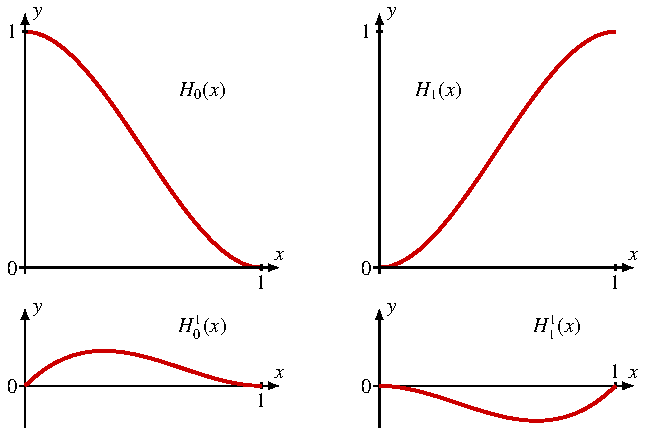
\includegraphics{chapters/030-nichtdiff/images/hermite.pdf}
\caption{Hermite-Polynome
\label{buch:nichtdiff:splines:fig:hermitepolynome}}
\end{figure}

Es müssen kubische Polynome auf dem Intervall $[x_k,x_{k+1}]$ konstruiert
werden, die vorgegebene Werte und Ableitungen in den Intervallenden haben.
Diese Aufgabe kann auf dem Intervall $[0,1]$ sofort gelöst werden,
wenn kubische Polynome auf dem bekannt sind, deren Werte der Funktion
und ersten Ableitungen an den Endpunkten $0$ sind mit Ausnahme jeweils eines,
der $1$ ist (Abbildung~\ref{buch:nichtdiff:splines:fig:hermitepolynome}).

\begin{satz}
\label{buch:nichtdiff:splines:satz:hermitebasis}
Die Polynome
\begin{align*}
H_0(x)   &=  (1+2x)(1-x)^2 = 2x^3-3x^2+1,
&&&
H_1(x)   &=      (3-2x)x^2 = -2x^3+3x^2,
\\
H_0^1(x) &=       x(1-x)^2 = x^3-2x^2+x,
&&\text{und}&
H_1^1(x) &=       (1-x)x^2 = x^3-x^2
\end{align*}
haben die Funktionswerte
\begin{align*}
H_0(0) &= 1,& H_1(0) &= 0,& H_0^1(0) &= 0,& H_0^1(1) &= 0,\\
H_0(1) &= 0,& H_1(1) &= 1,& H_0^1(0) &= 0,& H_0^1(1) &= 0
\intertext{und Werte der ersten Ableitungen}
H_0'(0) &= 0,& H_1'(0) &= 0,& H_0^{1\prime}(0) &= 1,& H_0^{1\prime}(1) &= 0,\\
H_0'(1) &= 0,& H_1'(1) &= 0,& H_0^{1\prime}(0) &= 0,& H_0^{1\prime}(1) &= 1
\end{align*}
an den Intervallenden.
Die zweiten Ableitungen der Polynome an den Intervallenden sind
\begin{align*}
H_0''(0) &= -6,& H_1''(0) &= \phantom{-}6,
&
H_0^{1\prime\prime}(0) &= -4,& H_1^{1\prime\prime}(0) &= -2,
\\
H_0''(1) &= \phantom{-}6 & H_1''(1) &= -6,
&
H_0^{1\prime\prime}(1) &=  \phantom{-}2,& H_1^{1\prime\prime}(1) &=  \phantom{-}4.
\end{align*}
\end{satz}

\begin{proof}
Die Behauptungen können durch Einsetzen der Argumente $0$ und $1$ in
die Polynome und ihre Ableitungen unmittelbar verifiziert werden.
\end{proof}

Mit den Polynomen von Satz~\ref{buch:nichtdiff:splines:satz:hermitebasis}
lässt sich die Aufgabe jetzt für ein Polynom auf einem Intervall
beliebiger Länge $l$ lösen.
Sei $P(x)$ ein kubisches Polynom.
Das Polynom $p(x)=P(x/l)$ ist ebenfalls kubisch und hat die Ableitungen
\[
p'(x) = P'(x/l)/l
\qquad\text{und}\qquad
p''(x) = P''(x/l)/l^2.
\]
Mit Hilfe einer Translation kann nun auch erreicht werden, dass die
verlangen Werten in den Punkten $x_k$ und $x_{k+1}$ angenommen werden.
Das Polynom
\(
p(x) = P((x-x_k)/(x_{k+1}-x_k))
\)
erfüllt
\begin{align*}
p(x_k)   &= P(0),                  &&          & p(x_{k+1})   &= P(1),               \\
p'(x_k)  &= P'(0)/(x_{k+1}-x_k),   &&          & p'(x_{k+1})  &= P'(1)/(x_{k+1}-x_k),\\
p''(x_k) &= P''(0)/(x_{k+1}-x_k)^2 &&\text{und}& p''(x_{k+1}) &= P''(1)/(x_{k+1}-x_k).
\end{align*}
Zur Vereinfachung der Notation bezeichnen wir die Länge der Teilintervalle
im Folgenden mit $m_k=x_{k+1}-x_k$.
Mit diesen Notation können wir jetzt für jedes Teilintervall $[x_k,x_{k+1}]$
ein kubisches Polynom konstruieren, welches die verlangten Werte und ersten
Ableitungen hat.

\begin{satz}
\label{buch:nichtdiff:splines:satz:polynom}
Das Polynom
\[
y_k(x)
=
y_k
H_0\biggl(\frac{x-x_k}{m_k}\biggr)
+
y_{k+1}
H_1\biggl(\frac{x-x_k}{m_k}\biggr)
+
s_k
m_k
H_0^1\biggl(\frac{x-x_k}{m_k}\biggr)
+
s_{k+1}
m_{k+1}
H_1^1\biggl(\frac{x-x_k}{m_k}\biggr)
\]
hat die Funktionswerte und ersten und zweiten Ableitungen
\begin{align*}
y_k(x_k)       &= y_k,
&
y_k'(x_k)      &= s_k,
&
y_k''(x_k)     &=
-\frac{6y_k}{m_k^2} + \frac{6y_{k+1}}{m_k^2}
-
\frac{4s_k}{m_k} - \frac{2s_{k+1}}{m_k},
\\
y_k(x_{k+1})   &= y_{k+1},
&
y_k'(x_k)      &= s_{k+1},
&
y_k''(x_{k+1}) &=
\phantom{-}\frac{6y_k}{m_k^2} - \frac{6y_{k+1}}{m_k^2}
+
\frac{2s_k}{m_k} + \frac{4s_{k+1}}{m_k}.
\end{align*}
\end{satz}

%
% Gleichungssystem für die Steigungen in den Stützstellen
%
\subsubsection{Gleichungssystem für die Steigungen in den Stützstellen}
Mit den im vorangegangenen Abschnitt gefundenen Polynome kann eine
Spline-Interpolationsfunktion konstruiert werden, sobald die ersten
Ableitungen der Funktion in den Stützstellen bekannt sind.
Diese müssen so gewählt werden, dass die daraus konstruierten
Polynome an den Stützstellen die gleichen zweiten Ableitungen haben.
In diesem Abschnitt soll ein Gleichungssystem hergeleitet werden, mit
denen diese ersten Ableitungen bestimmt werden können.

Seien $s_k=y'(x_k)$ die noch unbekannten Ableitungen in den Stützstellen.
Ausserdem sei $m_k = x_{k+1}-x_k$ die Länge des Intervalls $[x_k,x_{k+1}]$.
Die in Satz~\ref{buch:nichtdiff:splines:satz:polynom} konstruierten
Funktionen $y_k$ müssen in den Stützstellen die gleichen zweiten
Ableitungen haben, also
\[
y_{k-1}''(x_k) =  y_{k}''(x_k).
\]
Mit den Werten der zweiten Ableitung nach
Satz~\ref{buch:nichtdiff:splines:satz:polynom}
folgen jetzt die Gleichungen
\begin{align*}
\frac{6y_{k-1}}{m_{k-1}^2}
-
\frac{6y_{k}}{m_{k-1}^2}
+
\frac{2s_{k-1}}{m_{k-1}^2}
+
\frac{4s_k}{m_{k-1}^2}
&=
- \frac{6y_k}{m_k^2}
+
\frac{6y_{k+1}}{m_k^2}
-
\frac{4s_k}{m_k}
-
\frac{2s_{k+1}}{m_k}
\intertext{für $0<k<n$ und}
y''_0(x_0)
=
0
&=
-\frac{6y_0}{m_0^2}
+\frac{6y_1}{m_0^2}
-\frac{4s_0}{m_0}
-\frac{2s_1}{m_0}
\\
y''_n(x_n)
=
0
&=
\frac{6y_{n-1}}{m_{n-1}^2}
-
\frac{6y_n}{m_{n-1}^2}
+
\frac{2s_{n-1}}{m_{n-1}}
+
\frac{4s_n}{m_{n-1}}
\intertext{an den Intervallenden.
Bringen wir die unbekannten $s_k$ auf die linke Seite und alles
andere auf die rechte Seite erhalten wir}
\frac{2}{m_{k-1}}s_{k-1}
+
\biggl(
\frac{4}{m_{k-1}}
+
\frac{4}{m_k}
\biggr)s_{k-1}
+
\frac{2}{m_{k-1}^2}s_{k-1}
&=
-
\frac{6}{m_{k-1}^2}
y_{k-1}
+
\biggl(
\frac{6}{m_{k-1}^2}
-
\frac{6}{m_k^2}
\biggr)
y_k
+
\frac{6}{m_k^2}
y_{k+1}
\\
&=
\frac{6}{m_{k-1}^2}(y_k-y_{k-1})
+
\frac{6}{m_k^2}(y_{k+1}-y_k)
\intertext{für $0<k<n$ und}
\frac{4}{m_0}s_0
+
\frac{2}{m_0}s_1
&=
-\frac{6}{m_0^2}y_0
+\frac{6}{m_0^2}y_1
=
\frac{6}{m_0^2}(y_1-y_0)
\\
\frac{2}{m_{n-1}}s_{n-1}
+
\frac{4}{m_{n-1}}s_n
&=
-\frac{6}{m_{n-1}^2}y_{n-1}
+\frac{6}{m_{n-1}^2}y_n
=
\frac{6}{m_{n-1}^2}(y_n-y_{n-1})
\end{align*}
an den Intervallenden.
Dies ist ein lineares Gleichungssystem mit $n+1$ Gleichungen
für die $n+1$ Unbekannten $s_k$.
Wir schreiben es in Matrixform mit der Koeffizientenmatrix
\[
\renewcommand{\arraystretch}{1.9}
A=
\begin{pmatrix}
\displaystyle\frac{2}{m_0}
	&\displaystyle\frac{1}{m_0}
		&
			&
				&
					&
\\
\displaystyle\frac{1}{m_0}
	&\displaystyle\frac{2}{m_0}+\frac{2}{m_1}
		&\displaystyle\frac{1}{m_1}
			&
				&
					&
\\
	&\displaystyle \frac{1}{m_1}
		&\displaystyle \frac{2}{m_1} + \frac{2}{m_2}
			&\displaystyle \frac{1}{m_2}
				&
					&
\\
	&
		&\displaystyle\frac{1}{m_2}
			&\ddots
				&\ddots
					&
\\
	&
		&
			&\ddots
				&\ddots
					&\displaystyle\frac{1}{m_{n-2}}
\\
	&
		&
			&
				&\displaystyle\frac{1}{m_{n-2}}
					&\displaystyle\frac{2}{m_{n-1}}
\end{pmatrix}
\]
und der rechten Seite
\[
\renewcommand{\arraystretch}{1.9}
b
=
3
\begin{pmatrix}
\displaystyle
\frac{1}{m_0^2}(y_1-y_0)
\\
\displaystyle
\frac{1}{m_0^2}(y_1-y_0)
+
\frac{1}{m_1^2}(y_2-y_1)
\\
\displaystyle
\frac{1}{m_1^2}(y_2-y_1)
+
\frac{1}{m_2^2}(y_3-y_2)
\\
\vdots
\\
\displaystyle
\frac{1}{m_{n-2}^2}(y_{n-1}-y_{n-2})
+
\frac{1}{m_{n-1}^2}(y_n-y_{n-1})
\\
\displaystyle
\frac{1}{m_{n-1}^2}(y_n-y_{n-1})
\end{pmatrix}.
\]
Schreibt man die Ableitungen $s_k$ als Vektor $s$, können die Steigungen
durch Lösen der Gleichung
\[
As=b
\]
bestimmt werden.
Die spezielle {\em tridiagonale} Form der Matrix $A$
\index{tridiagonal}%
ermöglicht eine sehr effiziente Berechnung der Steigungen, den
Thomas-Algorithmus \cite{buch:thomas}.
\index{Thomas-Algorithmus}%
Sobald die Steigungen $s_k$ bestimmt sind, können die Funktionen
$y_k(x)$ mit Satz~\ref{buch:nichtdiff:splines:satz:polynom}
berechnet werden.

%
% Äquidistante Stützstellen
%
\subsubsection{Äquidistante Stützstellen}
Haben die Stützstellen gleichen Haben die Stützstellen Abstand, man
spricht von äquidistanten Stützstellen, dann sind alle $m_k$ gleich.
Wir schreiben $m=m_k$ für alle $k=0,\dots,n-1$.
In diesem Fall vereinfachen sich die Gleichungen beträchtlich, da
alle Nenner gleich sind.
Die Koeffizientenmatrix des Gleichungssystems ist
\[
A
=
\begin{pmatrix}
2 &1 &  &       &       &  \\
1 &4 &1 &       &       &  \\
  &1 &4 &1      &       &  \\[-3pt]
  &  &1 &\ddots &\ddots &  \\[-3pt]
  &  &  &\ddots &\ddots &1 \\
  &  &  &       &1      &2
\end{pmatrix}
\]
und die rechte Seite wird
\[
b
=
\frac{3}{m}
\begin{pmatrix}
y_1-y_0\\
y_2-y_0\\
y_3-y_1\\[-3pt]
\vdots\\
y_n-y_{n-2}\\
y_n-y_{n-1}
\end{pmatrix}
\]

\begin{beispiel}
Wir approximieren die Sinusfunktion mit Hilfe eines Splines mit zehn
Stützstellen.
\end{beispiel}

%
% Fehlerformel
%
\subsubsection{Fehlerformel}



\uebungsabschnitt

\aufgabetoplevel{chapters/030-nichtdiff/uebungsaufgaben}
\begin{uebungsaufgaben}
\uebungsaufgabe{301}
\end{uebungsaufgaben}
\enduebungsabschnitt

